\subsection{Traffic Demand Per Subscriber}\label{subsec:behavior}

To characterize the diurnal traffic demand observed at the ISP, we first 
calculate traffic demand per subscriber (table \ref{tab:eval-criteria}), and 
then plot the median and 95\%-ile of total usage over a week for both 
\treatment{} and \control{} sets (figure \ref{fig:traffic-demand-timeseries}).

We calculate demand by averaging the 
bytes transferred in uplink or downlink direction over the sample period (15 
minutes).\todo{ This allows us to capture both the average per subscriber 
demand at 
any time in a day, and the aggregate demand at the ISP over a longer period, 
such as a day or a week.}s

\begin{figure}[t]
\begin{minipage}{1\linewidth}
\centering
%
\begin{subfigure}[b]{0.5\linewidth}
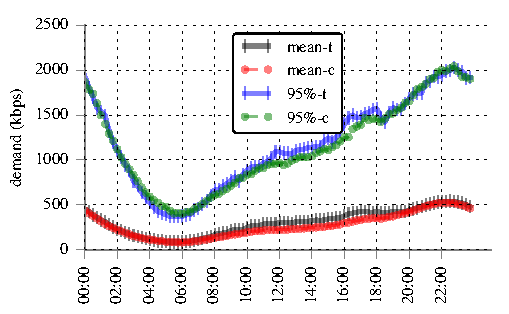
\includegraphics[width=\linewidth]{figures/weekday_demand_mean_perc95.pdf}
               \caption{Weekday traffic demand\label{fig:weekday-daily-usage}}
\end{subfigure}
%
\begin{subfigure}[b]{0.5\linewidth}
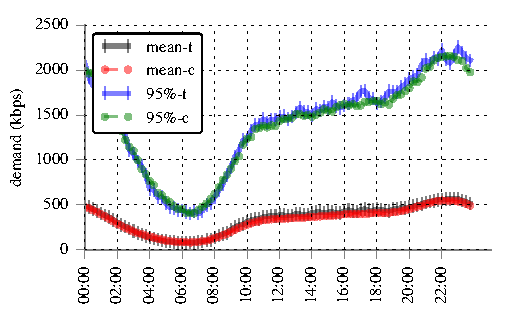
\includegraphics[width=\linewidth]{figures/weekend_demand_mean_perc95}
               \caption{Weekend traffic demand\label{fig:weekend-daily-usage}}
\end{subfigure}
%
\end{minipage}
\caption{Mean and 95th percentile traffic demand differs significantly on 
weekdays and weekends (including holidays). On weekdays, traffic demand 
increases monotonically from morning until prime-time in the evening. On 
weekends, there is a sharp rise in demand in the early morning, which 
plateaus until the next sharp rise during the evening prime-time hours.}
\label{fig:traffic-demand-timeseries}
\end{figure}



Figure \ref{fig:traffic-demand-timeseries} shows the aggregate data rate for 
weekdays and weekends day. 
\todo{ Results: mean and 95 percentile demand on weekdays and weekends }
We observed that the median traffic demand during 7:00 PM -- 7:00 AM is 
\todo{XXX} for both \treatment{} and \control{}. However, during off peak 
daytime (work) hours, between 7:00 AM -- 7:00 PM, the \treatment{} group has a 
median of \todo{XXX}, 20\% higher than the \control{} set.

\red{We observe that the rise to the peak prime time hour usage 
on weekdays is not plateaued like the pattern observed on weekends (and 
holidays). A generic (median) weekday aggregate usage consists of a rise in 
usage that starts early in the morning that builds up to the prime-time period, 
peaks, and then falls sharply. We do not observe a trough in mid afternoon 
(between 2:00 PM -- 6:00 PM), as is usually the case for overall usage observed 
at US Fixed access link providers \cite{sandvine20141h}.}
% EXPLAIN:
% LACK OF TROUGHS: users' behavior in higher tier bandwidth
% DISCREPANCY IN DAYTIME OFFPEAK: ???   


\begin{figure*}[t]
\begin{minipage}{1\linewidth}
\centering
%
\begin{subfigure}[b]{0.33\linewidth}
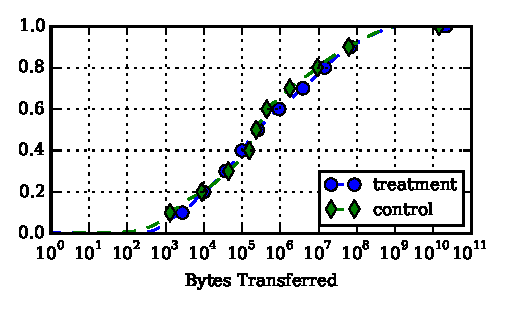
\includegraphics[width=\linewidth]{figures/cdf-all-bytes.pdf}
               \caption{Overall traffic demand\label{fig:CDF-data-rate}}
\end{subfigure}
%
\begin{subfigure}[b]{0.33\linewidth}
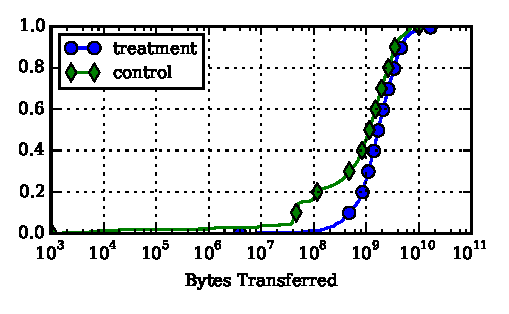
\includegraphics[width=\linewidth]{figures/cdf-per-device-max.pdf}
               \caption{Maximum traffic demand 
per subscriber\label{fig:CDF-data-rate-max}}
\end{subfigure}
%
\begin{subfigure}[b]{0.33\linewidth}
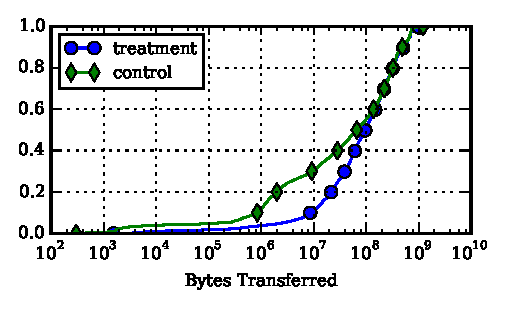
\includegraphics[width=\linewidth]{figures/cdf-per-device-perc95.pdf}
               \caption{Peak (95\%)
traffic demand per subscriber.\label{fig:CDF-data-rate-perc95}}
\end{subfigure}
%
\end{minipage}
\caption{The traffic demand throughout the dataset for both control and 
treatment is very similar. The daily maximum, and daily 95 percentile 
demand per subscriber increases due to the service upgrade. The 
higher 50 percent of the users with the heaviest link use in control increase 
their demands only by \red{xxx}. The other 50 percent of subscribers with the 
lower demand in the control group increase their demands two-fold with the 
upgrade.}
\label{fig:traffic-demand-cdf}
\end{figure*}

\todo{add an introductory/connecting para here}

A comparison of the aggregate traffic demand distribution of all devices 
and sample periods shows that the \treatment{} has no significant affect on the 
mean traffic demand. 
